%\documentclass[aps,preprint,amsmath,amssymb]{revtex4-1}% APS journal style
%\documentclass[aps,reprint,amsmath,amssymb,prl]{revtex4-1}% APS journal style prl physical review letters
\documentclass[aps,reprint,amsmath,amssymb,pra]{revtex4-1}% APS journal pra default
%\documentclass[aps,reprint,amsmath,amssymb,prl,longbibliography]{revtex4-1}% to show the title of the articles in the bibliography
\usepackage{graphicx}% Include figure files
\usepackage{dcolumn}% Align table columns on decimal point
\usepackage{bm}% bold math
\usepackage{hyperref}% add hypertext capabilities
%\bibliography{natbib}

\begin{document}
\title{A toy model to understand the dynamics of the vortical motions in turbulent boundary layers}
\author{J.C. Cuevas Bautista}
\email{jcc1@wildcats.unh.edu}
\affiliation{University of New Hampshire, Department of Mechanical Engineering, Durham 03824, USA.}
\date{\today}
\begin{abstract}
\noindent 
Recent studies indicate that the structure of the turbulent boundary layer at high Reynolds number (\textit{Re}) is composed of large uniform momentum zones segregated by fissures of concentrated vorticity. Experiments reveal that the dimensionless fissures thickness (scaled by boundary layer thickness) is $\mathcal{O}(1/\sqrt{Re})$ and the dimensionless streamwise velocity jump across a fissure scales with the friction velocity $\mathcal{O}(u_{\tau})$. A toy model that captures the essential elements of the turbulent boundary layer structure at high \textit{Re} is constructed to evaluate the long-time averaged flow statistics of the boundary layer. First, a ``master'' instantaneous  streamwise velocity profile in the wall-normal direction is constructed by placing a discrete number of fissuress across the boundary layer thickness. The number of fissures and their wall-normal locations follow scalings informed by the Mean Momentum Balance (MMB) theory. Next, the wall-normal positions of the fissures are allowed to randomly move in the wall-normal direction creating a statistically independent second instantaneous velocity profile. This process is then repeated to create an ensemble of instantaneous velocity profiles from which average statistics of the turbulent boundary layer can be computed and assessed. The statistics of the toy model are compared to statistics acquired in turbulent boundary layers at high \textit{Re}.
%Turbulent boundary layers are the result of complex interactions between a wide variety of scales present in the flow. Recent investigations indicates that the structure of turbulent boundary layers are physically composed of large uniform momentum zones segregated by fissures of concentrated vorticity which thickness scales with the Reynolds number $\delta^+$ as $1/\sqrt{\delta^+}$. The simplified model presented in this paper pretend to explain how these vortical fissures populate the turbulent boundary layer in special the inertial region. To do this Reynolds-Averaged Navier-Stokes equations must be simplified and solved, however in this model an alternative approach is considered. The thickness of vortical fissures is assumed negligible and the streamwise mean velocity profile is simulated as the result of the ensemble average of the instantaneous step velocity profiles. In addition the step profiles are modelled by zones of uniform velocity with discontinuous jumps of velocity (vortical fissures) along the wall normal position. Finally the positions of the vortical fissures are computed based on the Mean Momentum Balance theory (MMB) likewise the velocity increments. Results are computed for different Reynolds numbers and freestream velocities. The accurateness of the model is verified comparing the statistics of the first four moments of the turbulent mean velocity profile with the respective moments of the experimental data. variance is the stream-wise turbulent kinetic energy
\end{abstract}
\keywords{turbulent boundary layer, uniform momentum zones, vortical fissures and Mean Momentum Balance theory.}
%Words=207.
\maketitle
\section{\label{sec:nm} Numerical Methods}
A  step master stream-wise velocity profile is represented by a set of discrete steps uniformly spaced according with Eqs.~\ref{eq:upvel} and ~\ref{eq:yppos}, 
\begin{align}
U^+_{i+1}=&U^+_i+\phi_c^2 ln(\phi_c) \label{eq:upvel},\\
y^+_{i+1}=&\phi_c y^+_i. \label{eq:yppos}
\end{align}
These relationships are  derived from the MMB theory~\citep{Klewickimmb}, where Eq.~\ref{eq:upvel} determine the increments in the stream-wise normalized velocity $U^+$, the width of the steps in the $x$ coordinate and
Eq.~\ref{eq:yppos} determine the increments in the normalized wall normal position $y^+$, the height of the steps in the y coordinate (See Fig.~\ref{fig:master_profile}). The constant factor $\phi_c$ is given by $\phi_c=(1+\sqrt{5})/2$ and since the thickness of the
vortical fissures scales like $\mathcal{O}(1/\sqrt{Re})$, it is considered negligible at high $Re$. The initial wall normal position was set to $y^+_0=\phi_c\sqrt{\delta^+}$ in order to match with the onset of the logarithmic region according with the MMB theory and $U^+_0=0.5 U_{\infty}^+$ to be the half of the normalized free-stream velocity $U_{\infty}^+$. \\  

The last position $y_{N}^+$ of the vortical fissure and its associated velocity $U^+_{N}$ is bounded by the turbulent boundary layer thickness $\delta$ or its respective Reynolds number $\delta^+=\frac{\delta}{\nu/u_{\tau}}$, where $u_{\tau}=\sqrt{\tau_{\omega}/\rho}$ is the friction velocity ($\tau_{\omega}$ is the mean wall shear stress and $\rho$ is the mass density respectively) and $\nu$ is the kinematic viscosity. 
Fig.~\ref{fig:master_profile} 
\begin{figure}[b]
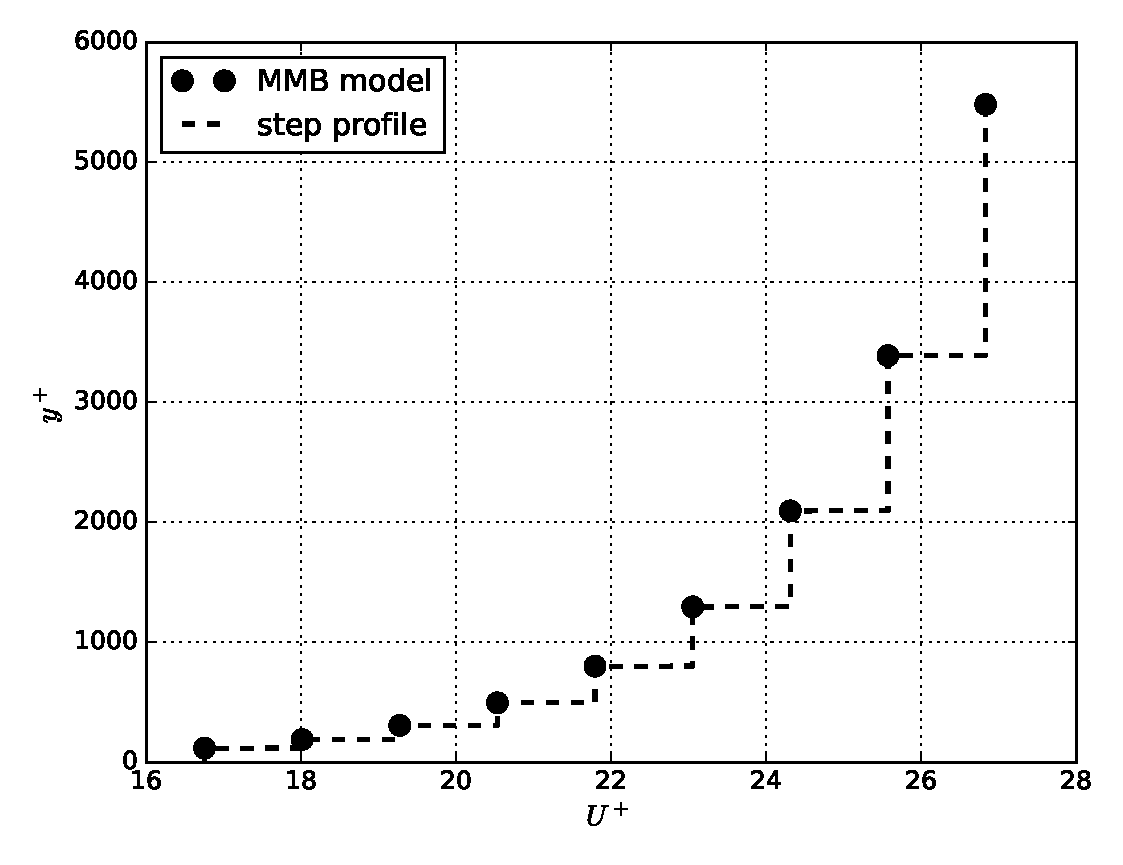
\includegraphics[scale=0.46]{figures/Master_step_profile}
\caption{\label{fig:master_profile} Step turbulence master profile for $\delta^+=5200$ and $U^+_{\infty}=26.5$.}
\end{figure} 
depicts the step master turbulent velocity profile with a grid of $5481$ linearly spaced positions in the wall normal direction each one associated to a streamwise velocity. The dot circles are the positions and velocities of the vortical fissures computed using Eqs.~\ref{eq:yppos} and \ref{eq:upvel} respectively. The zones of uniform momentum are created allocating the same velocity of the vortical fissure to the grid points between the previous vortical fissure and the current vortical fissure. This velocity remains characteristic for each vortical fissure, thus the number of vortical fissures establishes the number of uniform momentum zones. \\
Then instantaneous multiple velocity profiles are created by simulate a random motion in the wall normal direction  of the vortical structures. This is accomplished by add a Gaussian perturbation of the actual height of the uniform momentum zone to the current position of the vortical fissure (black dots in Fig.~\ref{fig:master_profile}) in the step turbulent master profile. Once the new wall normal positions have been computed, the grid velocity is filled with the attached velocity of each vortical fissure corresponding to their new wall normal positions. This physically means that the vortical fissures can cross each other through the turbulent boundary layer step profile generating zones of negative vorticity. Fig.~\ref{fig:mul_profiles} shows five instantaneous turbulent velocity step profiles, it can be seen how the vortical fissures changes their position trough the turbulent boundary layer for the different profiles. The time units in Fig.~\ref{fig:mul_profiles} are arbitrary, i.e. they just illustrate different instants of time. 
\begin{figure}[b]
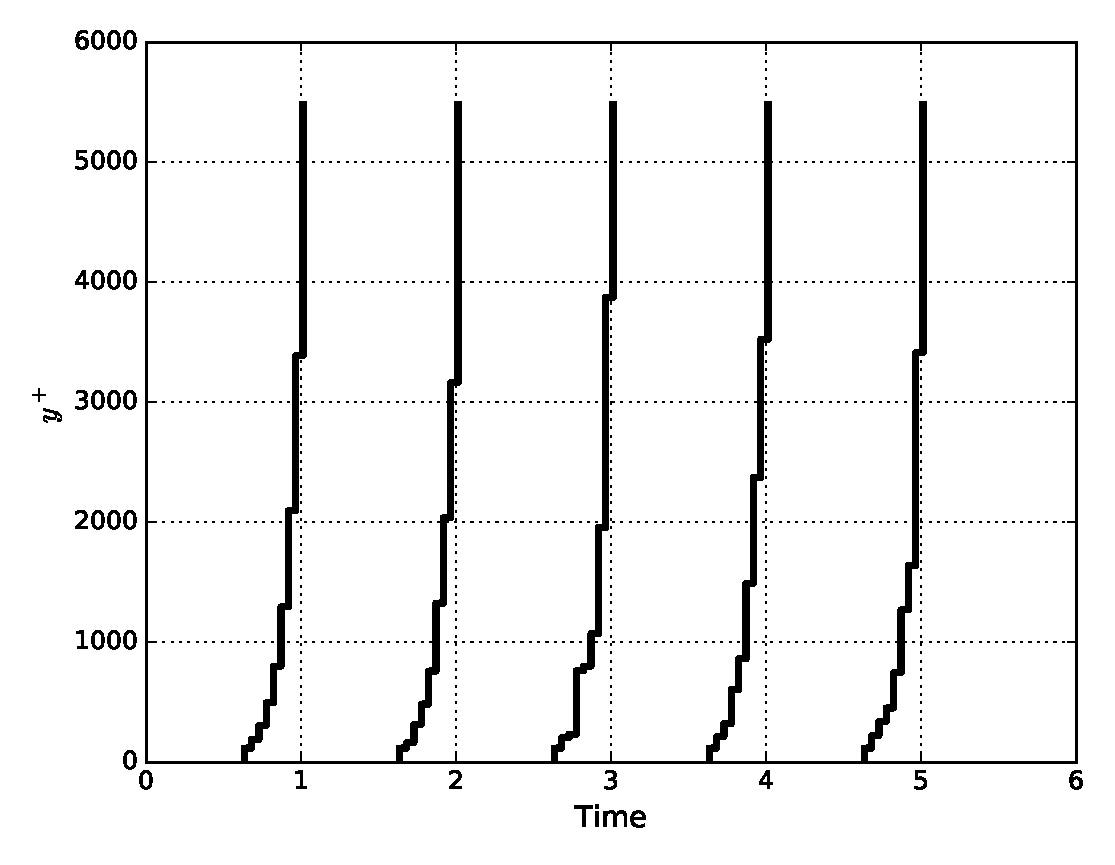
\includegraphics[scale=0.46]{figures/multiple_instantaneous_vprof}
\caption{\label{fig:mul_profiles} Multiple instantaneous velocity profiles with a gaussian perturbation of mean $\mu=0$ and standard deviation $\sigma=0.4$.}
\end{figure}
The multiple instantaneous step velocity profiles are considered independent events since they are the result of the Gaussian perturbation in the wall normal positions of the master profile. Thus to achieve statistical convergence the mean turbulent stream-wise velocity profile is constructed by average over 5000 independent realizations.
\section{Mean turbulent statistics analysis}
To prove the accurateness of our model, the high order moments such as the mean, variance, skewness and kurtosis of the mean turbulent streamwise velocity profile were computed. Like it was described in~\ref{sec:nm}, not only a Gaussian perturbation was used to randomize the positions of the vortical fissure but also an uniform distribution. The main purpose was explore the relationship between the perturbation distribution and the statistics of our model. This could give us some insight about how this process occurs in a real turbulent flow.
\subsection{Gaussian perturbation}
Multiple scenarios with different standard deviation were investigated for the Gaussian perturbation, however just two are presented here. They represent bad coherence with the experimental results $\sigma=0.4$ and good coherence with the experimental results $\sigma=1$, both with $\mu=0$. First scenario considers that the random variation in the position of the vortical fissures ranges between $-120\%$ and $120\%$ of their current positions, being $3\sigma$ events less likely. Fig~\ref{fig:mean_profile} is the mean turbulent velocity profile for the first scenario. It can be appreciated regions of relative uniform velocity along with small velocity jumps located close to the wall normal positions of the vortical fissures. This phenomena is known like clusterization and it is the result of the average of vortical fissures having the same velocities in the same wall normal positions.\\
\begin{figure}[b]
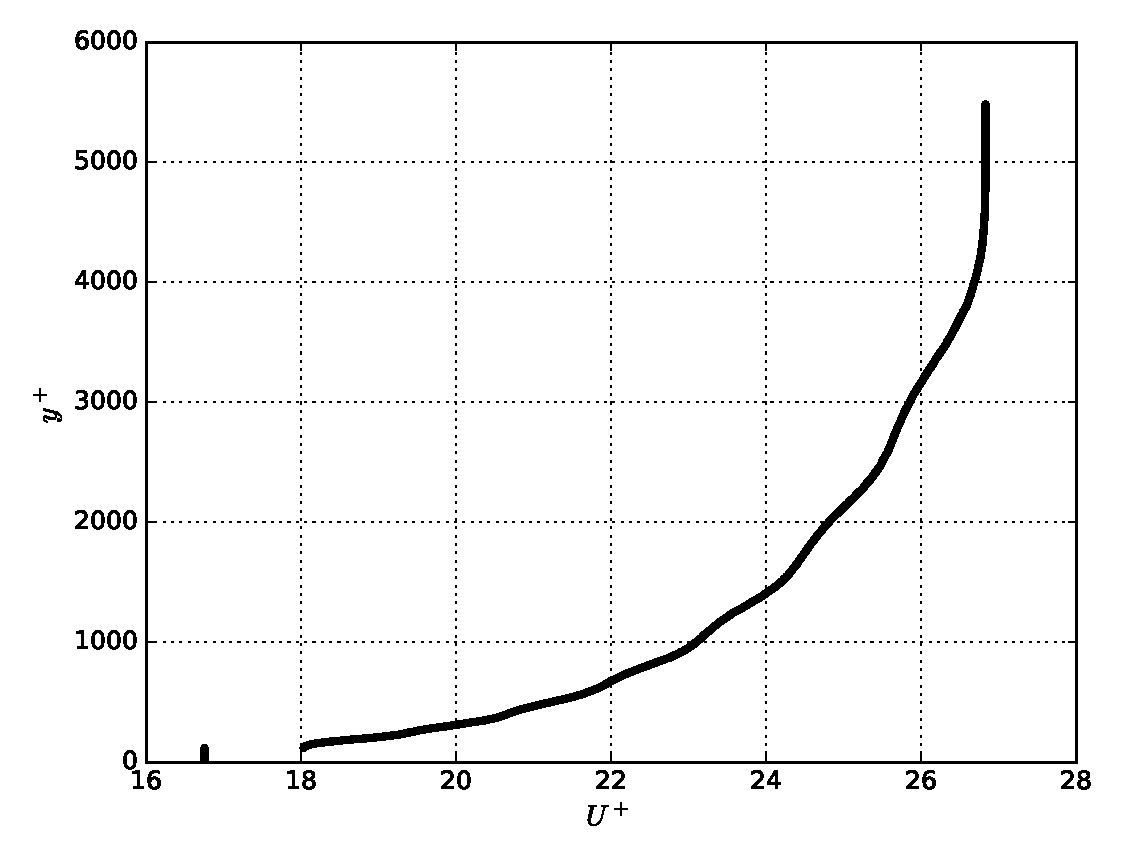
\includegraphics[scale=0.46]{figures/Master_averaged_step_profile_5000_assembles}
\caption{\label{fig:mean_profile} Mean turbulent stream-wise velocity profile for 5000 independent realizations with a Gaussian perturbation of $\mu=0$ and $\sigma=0.4$.}
\end{figure}

Fig~\ref{fig:varigaus}. shows the variance of the streamwise fluctuations for $5000$ independent realizations as a function of the wall normal position. Here the clusterization phenomena is more evident, this is one of the consequences which is known like pseudo-random number generators. Since the Gaussian random numbers are not totally independent but they are computed through a deterministic algorithm, wall normal positions can be populated with the same vortical fissures several times. It is also remarkable that for this scenario crossing vortical fissures are rarely observed. 

\begin{figure}[b]
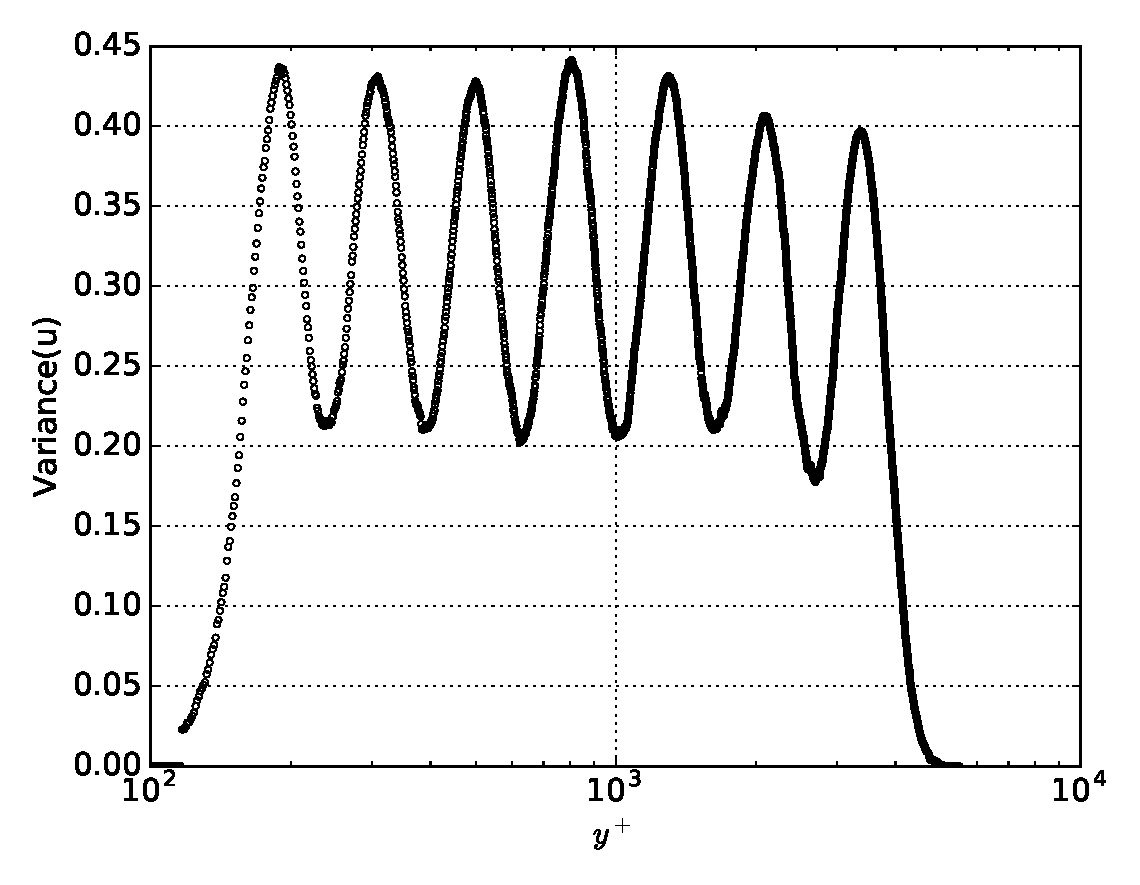
\includegraphics[scale=0.46]{figures/variance_5000_assembles}
\caption{\label{fig:varigaus} Stream-wise velocity variance for 5000 independent realizations with a Gaussian perturbation of $\mu=0$ and $\sigma=0.4$.}
\end{figure}
A semilogarithmic plot in the x-axis of the skewness for the streamwise fluctuations as a function of the wall normal position is shown in Fig~\ref{fig:skewgaus}. It shows the right tendency for wall normal positions close to the wall and in the boundary edge. However in the logarithmic region the skewness oscillates around the Gaussian value, these
rapid variations are caused by clustering effect. Unlike the skewness (Fig~\ref{fig:skewgaus}), the stream-wise velocity kurtosis oscillations are higher if they are compared with the Gaussian distribution where the kurtosis is equal to 3. This behaviour does not reproduce accurately the turbulence statistics and thus we explore higher values of $\sigma$ in the Gaussian perturbation.\\

\begin{figure}[tb]
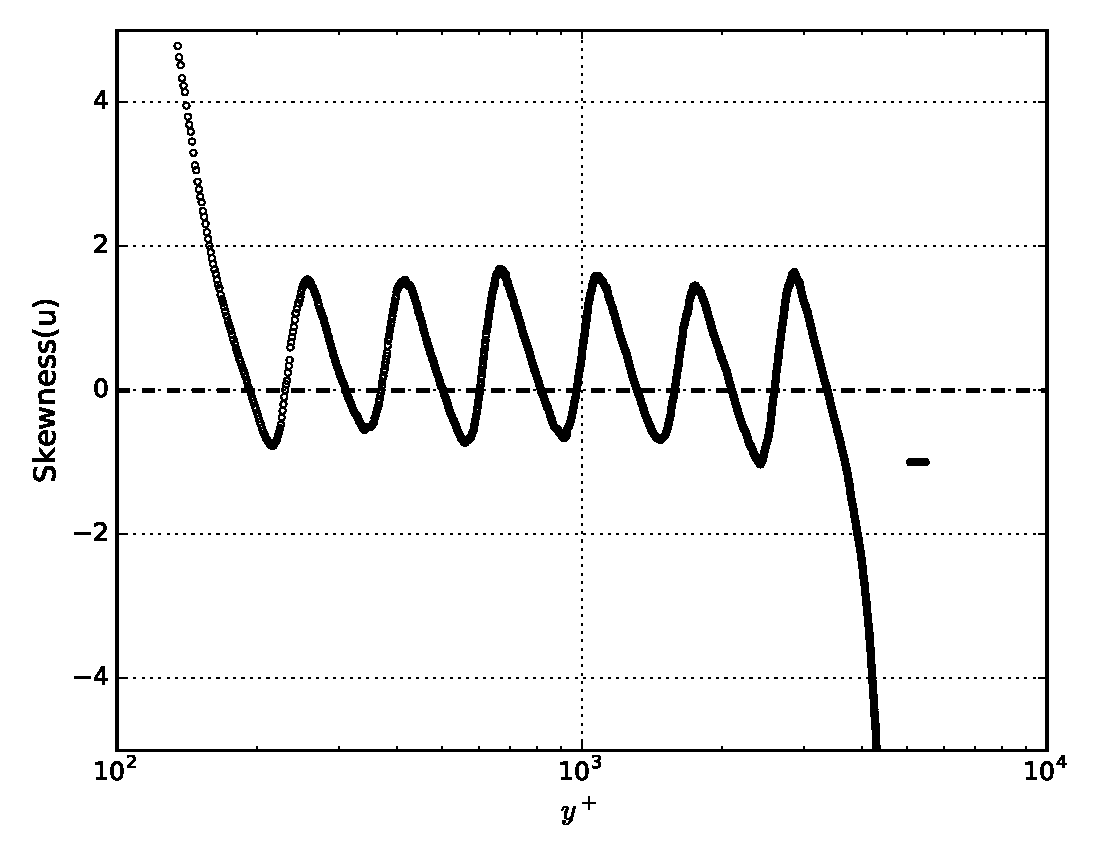
\includegraphics[scale=0.46]{figures/skewness_5000_assembles}
\caption{\label{fig:skewgaus} Stream-wise velocity skewness for 5000 independent realizations with a Gaussian perturbation of $\mu=0$ and $\sigma=0.4$ (open circles). The skewness for a Gaussian distribution is plotted in dotted lines as a reference.}
\end{figure}
In the second scenario $\sigma=1$, hence the random motion of the vortical fissures range between $-300\%$ and $300\%$ of their respective height of the step (see~\ref{sec:nm}). Fig~\ref{fig:mp_gau100}. shows a smoother profile compared with the first scenario where clustering effect was evidenced. These mean velocity profile exhibit the right trend for $\delta^+=5200$, the constant velocity close to the wall ($y^+=0-118$) is a consequence of the boundary conditions where the first step velocity is held fixed.
\begin{figure}[tb]
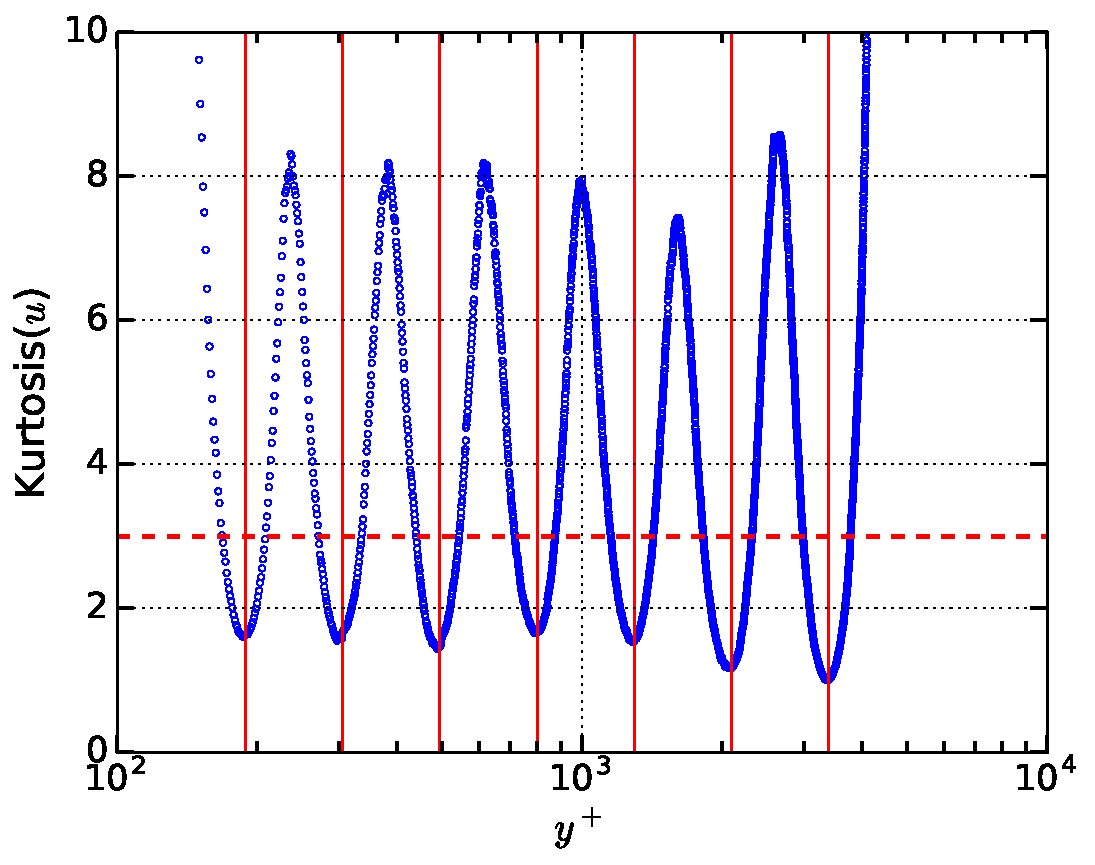
\includegraphics[scale=0.46]{figures/kurtosis_5000_assembles}
\caption{\label{fig:kurt} Stream-wise velocity kurtosis for 5000 independent realizations with a Gaussian perturbation of $\mu=0$ and $\sigma=0.4$ (open circles). The kurtosis for a Gaussian distribution is plotted in dotted lines as a reference.}
\end{figure}
In addition to the mean, the second, third and fourth order moments are also computed for this scenario. The stream-wise velocity variance as a function of $y^+$ is shown in Fig~\ref{fig:varigaus100}.\\ 
It can be seen that the variance start to exhibit the right trend, namely zero near to the wall with its maximum value in the onset of the logarithmic region and then decrease almost logarithmically toward the boundary layer edge. 
\begin{figure}[tb]
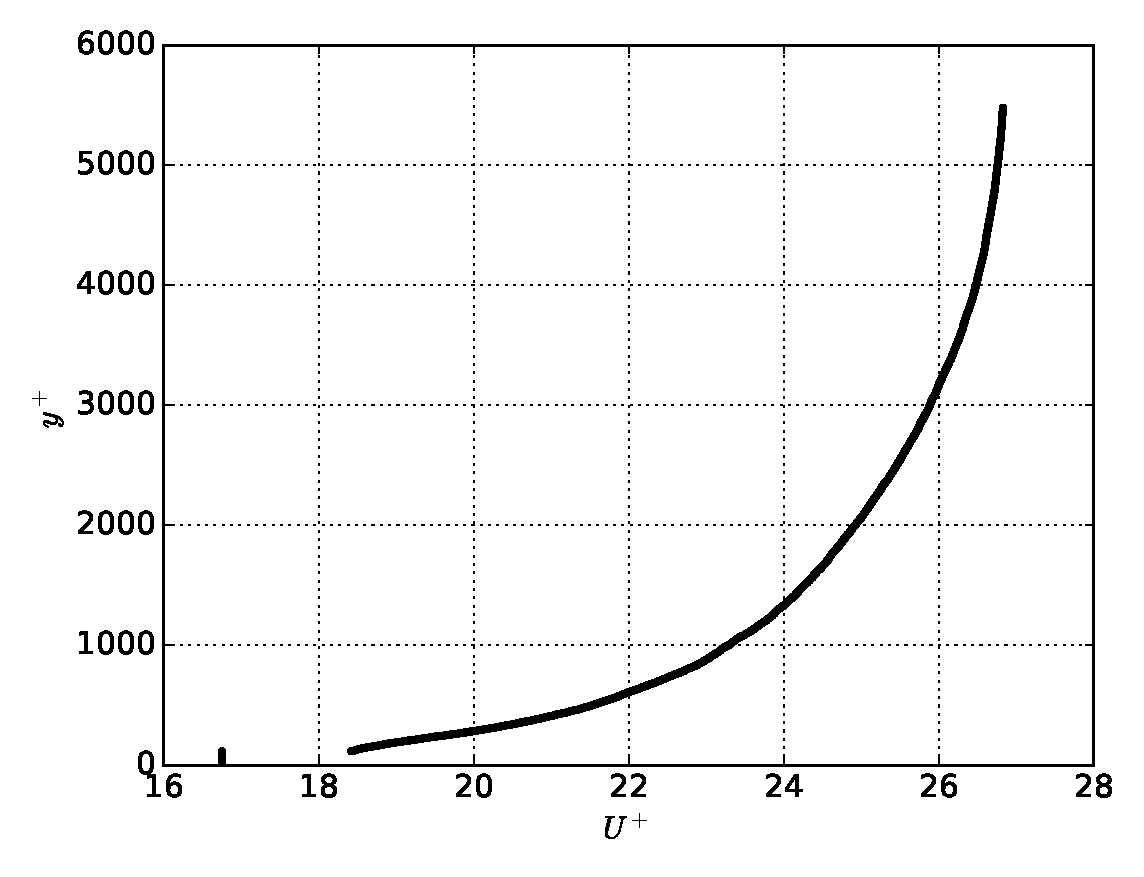
\includegraphics[scale=0.46]{figures/Master_averaged_step_profile_5000_assembles_gaus100}
\caption{\label{fig:mp_gau100} Mean turbulent stream-wise velocity profile for 5000 independent realizations with a Gaussian perturbation of $\mu=0$ and $\sigma=1$.}
\end{figure}
Also note that there is not evidence of clustering effect, since a wider range in the vertical perturbations allow the vortical fissures to cross through the boundary layer creating a more homogeneous distribution of the stream-wise velocity. 
\begin{figure}[b]
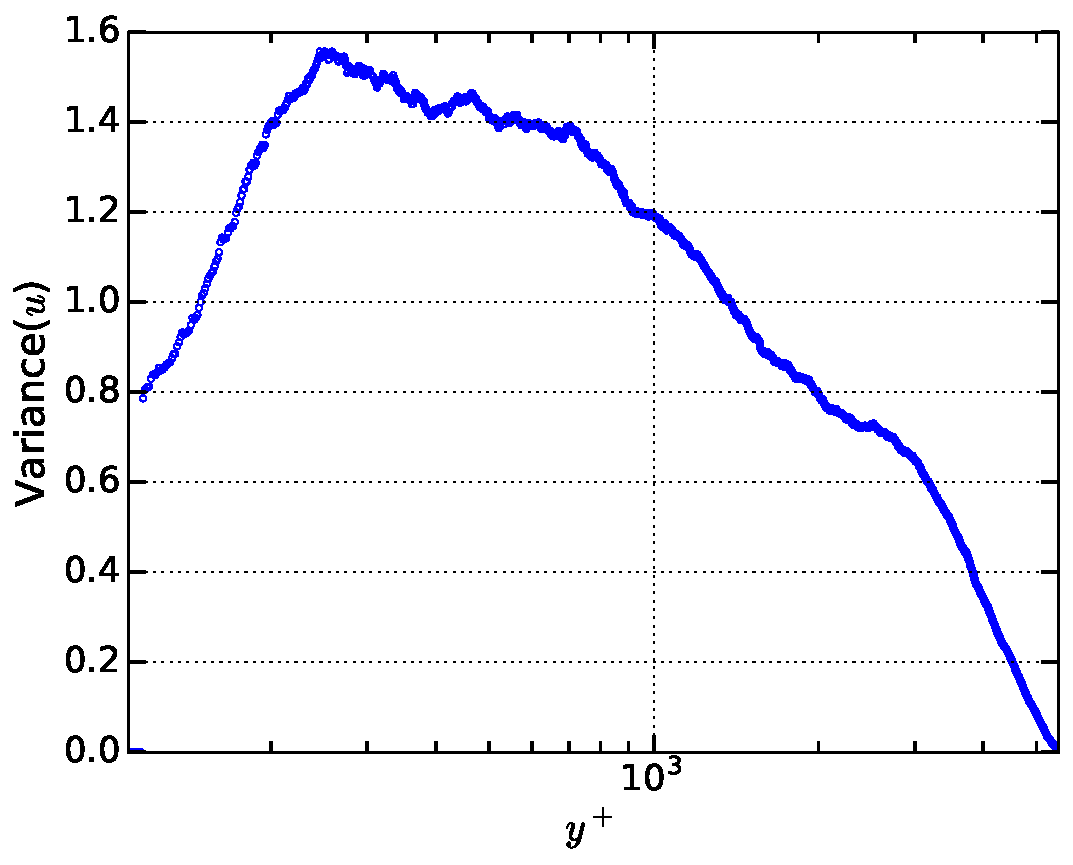
\includegraphics[scale=0.46]{figures/variance_5000_assembles_gauss100}
\caption{\label{fig:varigaus100} Stream-wise velocity variance for 5000 independent realizations with a Gaussian perturbation of $\mu=0$ and $\sigma=1$.}
\end{figure}
Fig~\ref{fig:skewgaus100} shows the skewness for $\sigma=1$, it can be seen how the skewnees has its maximum positive value close to the wall and then when it is approaching to the log region it exhibits a Gaussian behaviour to raise up to its maximum negative value at the end of the logarithmic region.  Unlike the experimental results for a turbulent skewness, the boundaries don't have the right trend. This is caused mainly because the first and last step in our model are not being perturbed. Further investigation is necessary to establish the proper boundary conditions in order to reproduce the real tendency in the boundaries for the skewness.
\begin{figure}[tb]
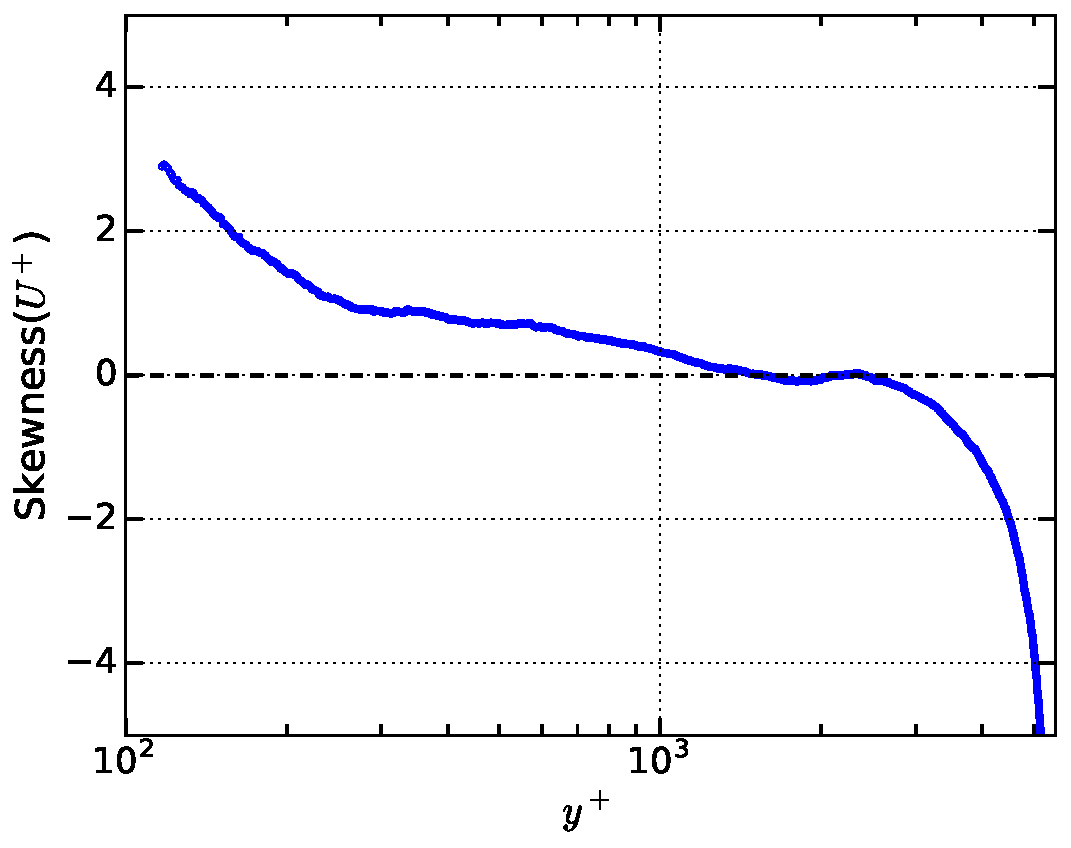
\includegraphics[scale=0.46]{figures/skewness_5000_assembles_gauss100}
\caption{\label{fig:skewgaus100} Skewness of streamwise velocity fluctuations for 5000 independent realizations with a Gaussian perturbation of $\mu=0$ and $\sigma=1$ (open circles). The skewness for a Gaussian distribution is plotted in dotted lines as a reference.}
\end{figure}
A similar pattern can be seen for the streamwise kurtosis (Fig~\ref{fig:kurtgaus100}), where the tendency in the boundaries does not reproduce accurately the experimental results. However in the logarithmic region the kurtosis exhibits a subgaussian trend just as the real data does. For $y^+=\delta^+$ is expected that the kurtosis reach its maximum value and
then decays in the free-stream region for the flow. This suggest that a different distribution can be used to perturb the position of the vortical fissures which edges decays smoother than the gaussian distribution. 
\begin{figure}[tb] 
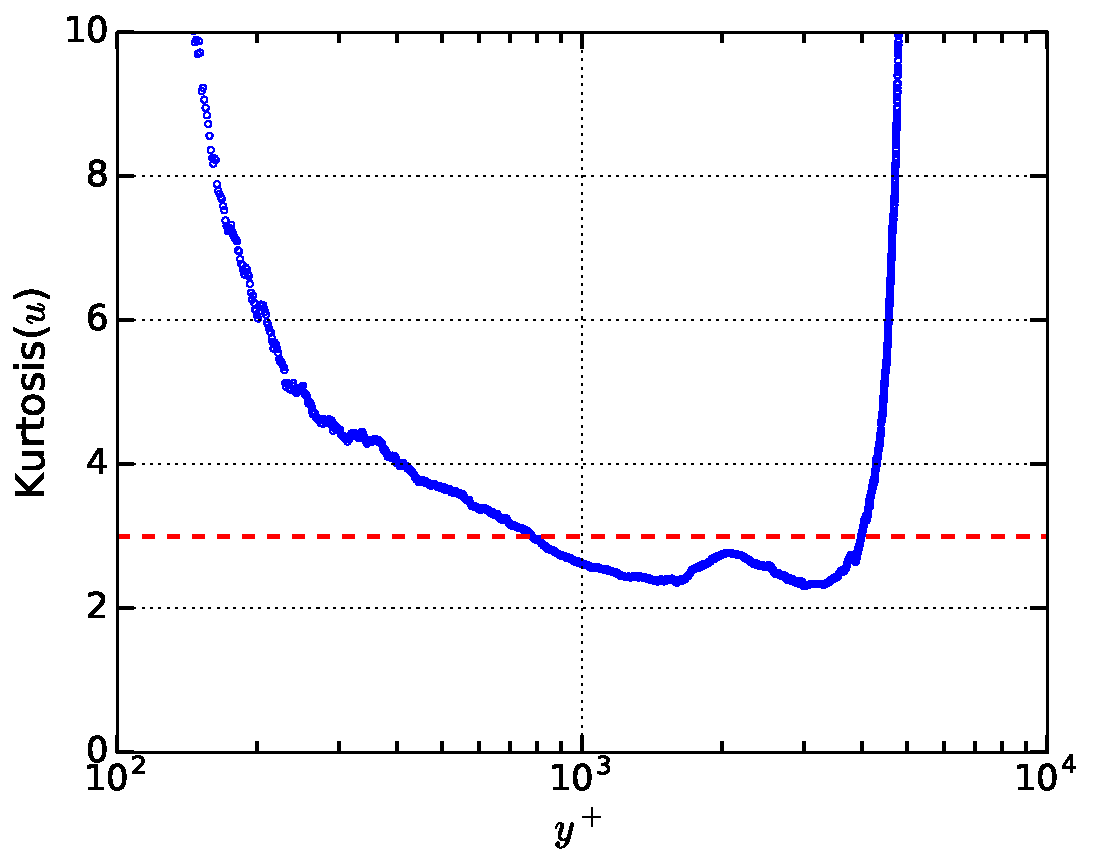
\includegraphics[scale=0.46]{figures/kurtosis_5000_assembles_gauss100}
\caption{\label{fig:kurtgaus100} Kurtosis of streamwise velocity fluctuations for 5000 independent realizations with a Gaussian perturbation of $\mu=0$ and $\sigma=1$ (open circles). The kurtosis for a Gaussian distribution is plotted in dotted lines as a reference.}
\end{figure}
Thus a uniform distribution is explored in the next section, which attempts to avoid this undesirable tendency in the boundaries of the turbulent boundary layer.
\subsection{Uniform distribution}
In order to allow vortical fissure crossing a uniform distribution between $-130\%$ and $130\%$ of the height of the step was selected. Fig~\ref{fig:mp_un130}  shows the streamwise velocity profile for this perturbation. Unlike Fig~\ref{fig:mean_profile}, the jumps in the velocity profile seems to have a more straight slope. 
\begin{figure}[b]
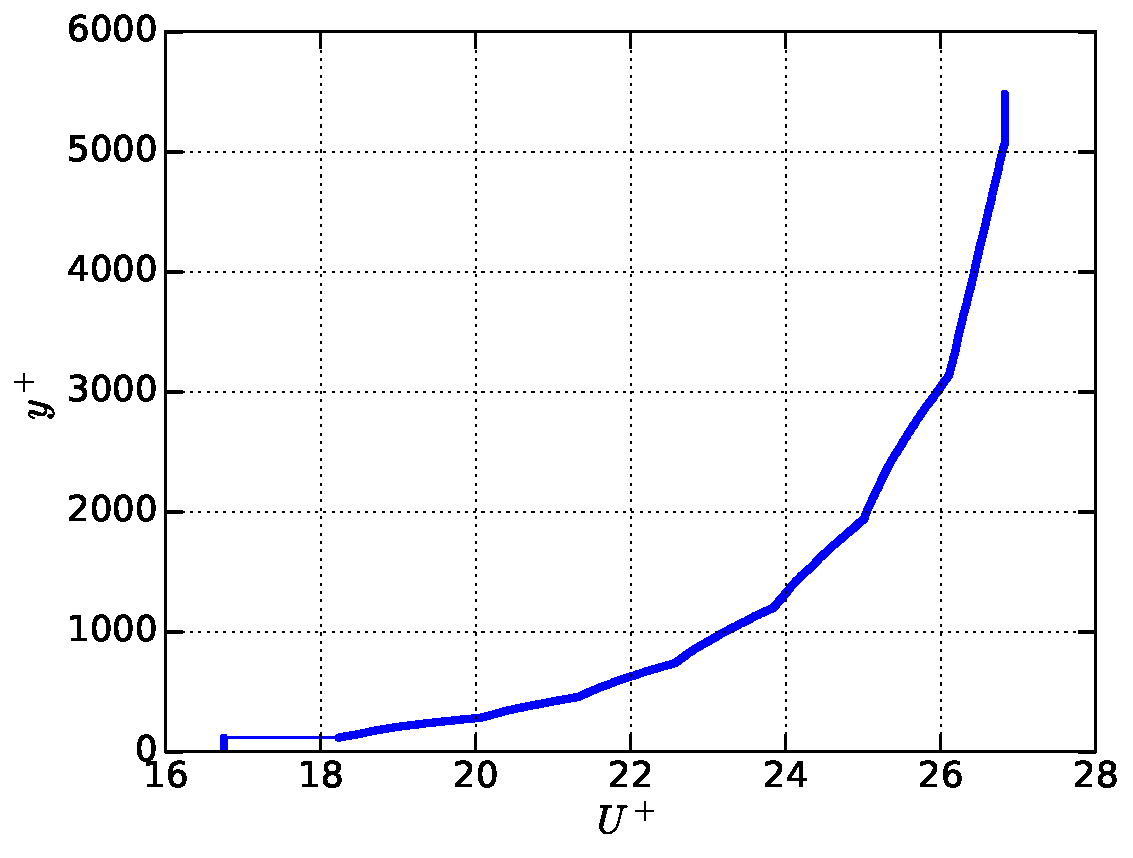
\includegraphics[scale=0.46]{figures/Master_averaged_step_profile_5000_assembles_un130}
\caption{\label{fig:mp_un130} Mean turbulent stream-wise velocity profile for 5000 independent realizations with an uniform perturbation of $\pm 130$.}
\end{figure}

     
%\nocite{*}
\bibliography{Aps_template2}% Produces the bibliography via BibTeX.
\end{document}
